\documentclass[conference]{IEEEtran}
\IEEEoverridecommandlockouts
% The preceding line is only needed to identify funding in the first footnote. If that is unneeded, please comment it out.
\usepackage{cite}
\usepackage{amsmath,amssymb,amsfonts}
\usepackage{algorithmic}
\usepackage{graphicx}
\usepackage{textcomp}
\usepackage{xcolor}
\usepackage{float}
\usepackage{subfigure}
\usepackage{subfig}
\graphicspath{{../figures/}}


\def\BibTeX{{\rm B\kern-.05em{\sc i\kern-.025em b}\kern-.08em
    T\kern-.1667em\lower.7ex\hbox{E}\kern-.125emX}}
\begin{document}


\title{Design of $4\times 4$ multiplier from schematic to layout
\thanks{Identify applicable funding agency here. If none, delete this.}
}

\author{\IEEEauthorblockN{1\textsuperscript{st} YUAN Tong}
\IEEEauthorblockA{\textit{School of Microelectronic} \\
\textit{Southern University of Science and Technology}\\
Shenzhen, China \\
yuant2018@mail.sustech.edu.cn}
\and
\IEEEauthorblockN{2\textsuperscript{nd} FAN Qinyuan}
\IEEEauthorblockA{\textit{School of Microelectronic} \\
\textit{Southern University of Science and Technology}\\
Shenzhen, China \\
fanqy2018@mail.sustech.edu.cn}
}

\maketitle

\begin{abstract}
    In this paper a low power and high speed 4X4 multiplier is designed using TSMC 0.18nm CMOS Technology. The important factors in VLSI Design are power, area, speed and design time. Now-a-days, power and speed has become a crucial factor in Digital Signal Processor (DSP) Applications. However, different optimization techniques are available in the digital electronic world. The proposed approach a Low power and high speed Multiplier Design based on Modified Column bypassing technique mainly used to reduce the switching power activity. While this technique offers great dynamic power savings, due to their interconnection. In this work, a low power and high speed multiplier with Hybridization scheme is presented. This scheme is combination of booth encoder algorithm and column bypass technique is called modified column bypassing scheme. The simulations are performed in 0.18µm CMOS Technology in Cadence Virtuoso tools with operating voltage ±1.8v.
\end{abstract}

\begin{IEEEkeywords}
    Multiplier, CMOS, Column Bypassing, Digital Signal Applications (DSP), Row Bypassing, Booth encoder
\end{IEEEkeywords}

\section{Introduction}

% In the introduction, students are asked to give a short introduction on the subject. This would include: A brief background study related to the topic; Motivation of the project; Possible application of the design.

As one of the key components of modern CPU, multiplier is a widely studied computer architecture which take the responsbility of most of the calculation operation in computer. Currently widely used multiplier inculding Booth multiplier, Sequential multiplier, combinational multiplier, Wallace tree multiplier \cite{a1}. The performance of the multiplier is a key fact that will greatly affect the performance of processors, so the design of a small, fast and energy efficiency multiplier is a prior problem we need to pay attention to today.

In this report, we will demostrate the design procedure of the $4 \times 4$ multiplier. In secition \ref{basic}, we will introduce the design of basic components including NAND gate, AND gate, XOR gate and invertor then we assemble them into main componet of a multiplier, half adder and full adder. In section \ref{Assemble} we will build the multiplier and the performance of the multiplier will be tested in section \ref{test}.

\section{Our Problem and design idea}

% Explain briefly the objectives of the project. For example the design of low power array multiplier, with minimum delay and minimum silicon area. Explain how you achieve these objectives.

In this project we are assigned to design a classcial $ 4 \times 4 $ bit multiplier as small and fast as possible, and we also wish we could use high level design to increase the design speed. To achieve our goal, we will focus on the following design principles. Firstly, we will minimize the width of each components and the space between them under the constrain of design rule, that will help us achiveve the minimum space. Secondly, we need to aviod using high layer of metal which is the main cause of delay. Finally we can find the minimun kinds of components we need by apply top-to-down design. 

To design the multiplier start from the high level structure of the multiplier, as shown in Figure \ref{High level structure of 4x4 multiplier}, a multiplier consists of half adder, full adder, and AND Gate, and a step futher, we can move our attention to the structure of full adder and half adder. In Fig \ref{Half adder} and \ref{Full adder}, we can see the two differnt kinds of adders are consist of NAND Gate, XOR Gete, and AND Gate, while and gate can be divided into NAND Gate and invertor, so what we need is NAND Gate, Inverter and XOR Gate, though XOR Gate can be divided into more simple gates, but to reduce the space, we will design the XOR Gate as a single component.

\begin{figure}[h]
    \centering
    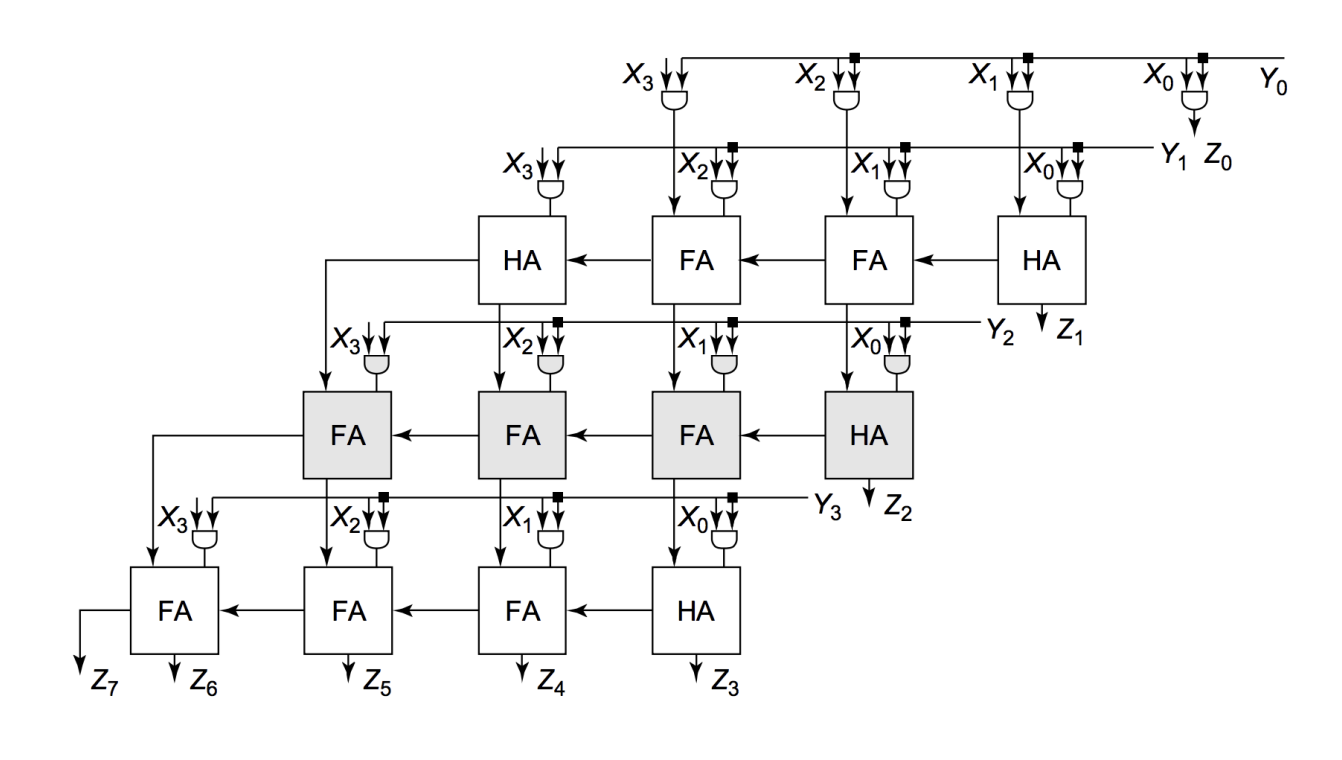
\includegraphics[width=0.9\linewidth]{4x4_multiplier.png}
    \caption{High level structure of 4x4 multiplier}
    \label{High level structure of 4x4 multiplier}
\end{figure} 

\begin{figure}[h]
    \centering
    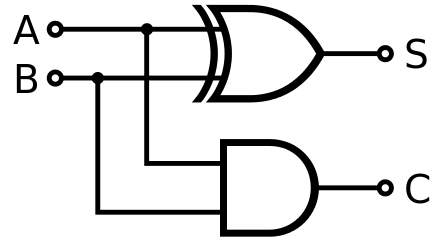
\includegraphics[width=0.45\linewidth]{half_adder.png}
    \caption{Half adder}
    \label{Half adder}
\end{figure}

\begin{figure}[h]
    \centering
    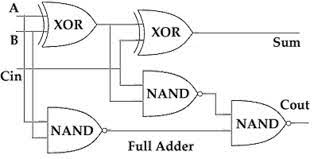
\includegraphics[width=0.6\linewidth]{full_adder.jpeg}
    \caption{Full adder}
    \label{Full adder}
\end{figure}

% In this section students should first start by describing the global architecture with clear drawing(s). A top - down description is encouraged. In this section students are encouraged to go through the different circuit diagrams as well as the sizing of the transistors, simulation layout and post-layout simulation. Students are encouraged to put more emphasis on how they are taking care of the objectives set. This section should also include the analysis of the critical delay, study of the floor-planning for the different blocks, and the final circuit together with the physical layout and its verification. The details that should be covered in this section include the following parts with tables and descriptions.

\section{Design and verication of basic components}

% You need to develop a library of basic (standard) cells that are used for the multiplier design. All the components in the library (inverters and more complex gates that are needed for the final multiplier design) must be briefly introduced. Prepare a Table with the transistors sizes (both width and length in micrometers), output low-to-high propagation delay, and output high-to-low propagation delay of each basic cell that is used in the multiplier design. If you have different sizes of the same type of logic gate, you need to report the size and delay of each different sized gate in your library. Produce the delay data using post-layout simulation for each type of gate. Add the Table in your report. Apply an input signal with rise and fall times of 0.2 ns (10% to 90% signal transition time) for measuring the delays. For each basic gate, report three different delays with three different extrinsic load capacitors: C1 = 15 fF, C2 = 8*C1, and C3 = 64*C1. Discuss the relationship between delay and extrinsic load capacitance in the report. How does this relationship change as you go from a CMOS inverter to more complex gates with more than one input? Provide your answers in the report.

\label{basic}

\subsection{Inverter}

The simpliest structure is Inverter consists of a pmos and a nmos as shown in Fig \ref{Schematic of Inverter}, they all have 0.18um in length, which is the minimun length of gate under 0.18 um TSMC technology, and after a balence between space and speed, we choose 4um as the width of pmos and 1.6um as the width of the nmos, to make sure all the gates perform well, the size of other gates will equivlent the inverter.

\begin{figure}[H]
    \centering
    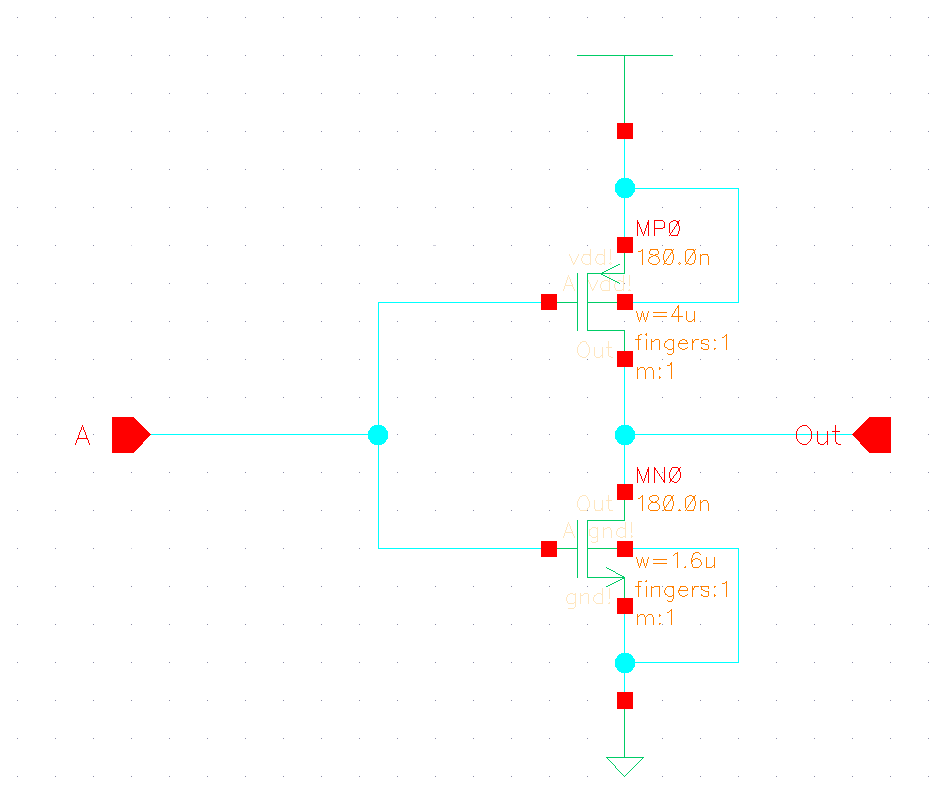
\includegraphics[width = 0.6\linewidth]{inv_schematic}
    \caption{Schematic of Inverter}
    \label{Schematic of Inverter}
\end{figure}

Then we will test the performance of the inverter, we add three different extrinsic load capacitors: C1 = 15 fF, C2 = 8*C1, and C3 = 64*C1 to the output of the inverter and test its delay, the result is listed in Table \ref{The delay of inverter}. To measure the propagation delay, we will 

\begin{table}[h]
    \caption{The delay of inverter}
    \begin{center}
        \begin{tabular}{|c|c|c|c|c|c|c|}
            \hline
            \textbf{Cap} & \multicolumn{2}{|c|}{15f F} & \multicolumn{2}{|c|}{120f F} & \multicolumn{2}{|c|}{960f F} \\
            \hline
            \textbf{State} & Up & Down & Up & Down & Up & Down \\
            \hline
            \textbf{Delay(ns)} & 0.080 & 0.071 & 0.194 & 0.179 & 1.080 & 0.988 \\
            \hline
        \end{tabular}
    \end{center}
    \label{The delay of inverter}
\end{table}

\subsection{NAND Gate}

NAND Gate is one of the most important basic gates, to make the gate equivlent to inverter we choose 4um as the width of the PMOS, and 3.2um as the width of NMOS.

\begin{figure}[H]
    \centering
    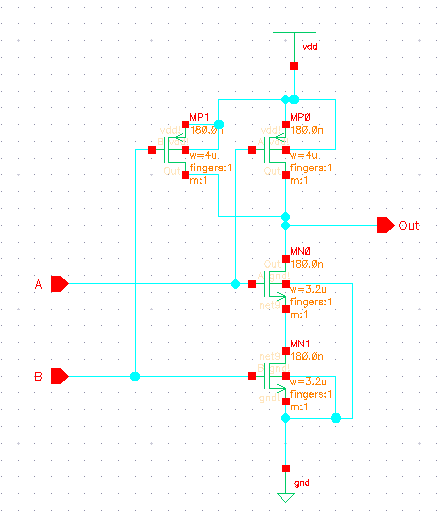
\includegraphics[width = 0.7\linewidth]{nand2_schematic.png}
    \caption{Schematic of NAND Gate}
    \label{Schematic of NAND Gate}
\end{figure}

The performance of NAND Gate will be tested under the same method as Inverter.

\begin{table}[h]
    \caption{The delay of NAND Gate}
    \begin{center}
        \begin{tabular}{|c|c|c|c|c|c|c|}
            \hline
            \textbf{Cap} & \multicolumn{2}{|c|}{15f F} & \multicolumn{2}{|c|}{120f F} & \multicolumn{2}{|c|}{960f F} \\
            \hline
            \textbf{State} & Up & Down & Up & Down & Up & Down \\
            \hline
            \textbf{Delay(ns)} & 0.086 & 0.059 & 0.197 & 0.147 & 1.076 & 0.785 \\
            \hline
        \end{tabular}
    \end{center}
    \label{The delay of NAND}
\end{table}

\subsection{AND Gate}

To make things more simplfied, we use a inverter and a NAND Gate to assemble an AND Gate, so the size of MOS transistors in AND Gate can be refered from the size of NAND Gate and Inverter.

\begin{figure}[H]
    \centering
    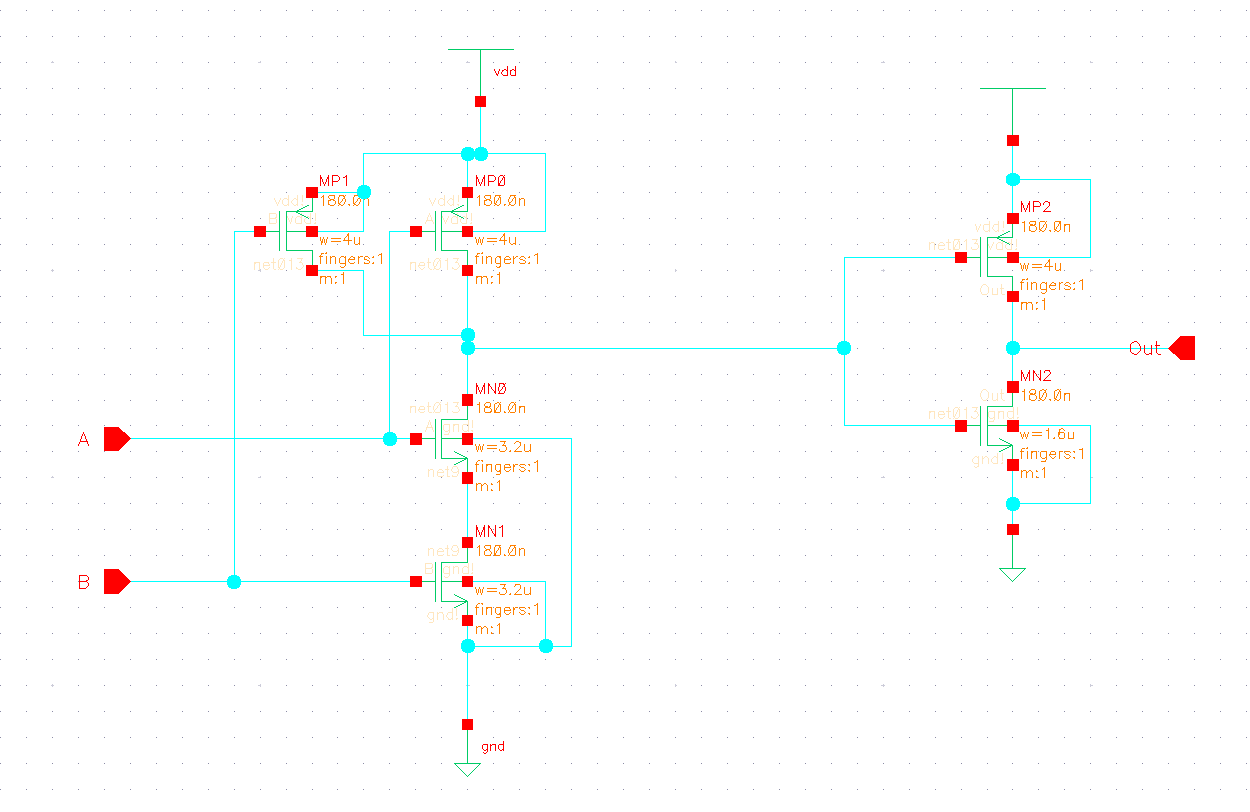
\includegraphics[width = 0.9\linewidth]{and2_schematic.png}
    \caption{Schematic of AND Gate}
    \label{Schematic of AND Gate}
\end{figure}

The performance of AND Gate will be tested under the same method as Inverter.

\begin{table}[h]
    \caption{The delay of AND Gate}
    \begin{center}
        \begin{tabular}{|c|c|c|c|c|c|c|}
            \hline
            \textbf{Cap} & \multicolumn{2}{|c|}{15f F} & \multicolumn{2}{|c|}{120f F} & \multicolumn{2}{|c|}{960f F} \\
            \hline
            \textbf{State} & Up & Down & Up & Down & Up & Down \\
            \hline
            \textbf{Delay(ns)} & 0.124  & 0.152 & 0.238 & 0.261 & 1.003 & 1.068 \\
            \hline
        \end{tabular}
    \end{center}
    \label{The delay of AND}
\end{table}

\subsection{XOR Gate}

For XOR Gate, we have same MOS size as Inverter, as all the PMOSs have width 4um and NMOSs have width 1.6nm.

\begin{figure}[H]
    \centering
    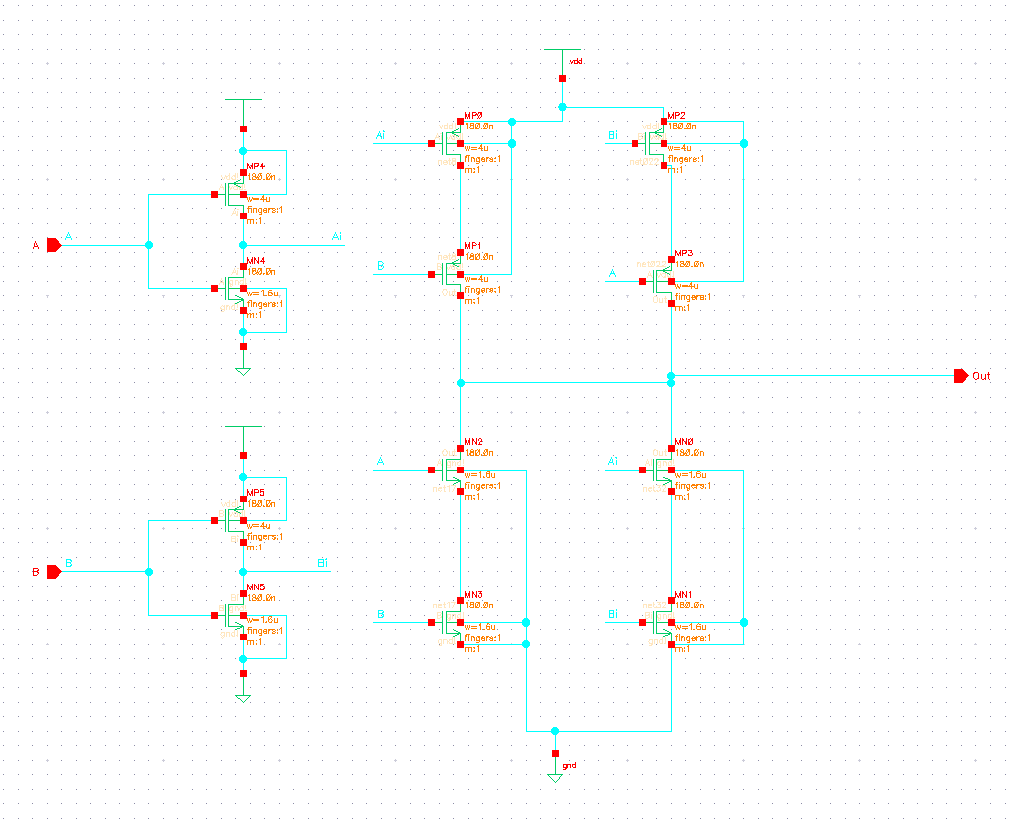
\includegraphics[width = 0.9\linewidth]{xor2_schematic.png}
    \caption{Schematic of XOR Gate}
    \label{Schematic of XOR Gate}
\end{figure}

\begin{figure}[H]
    \centering
    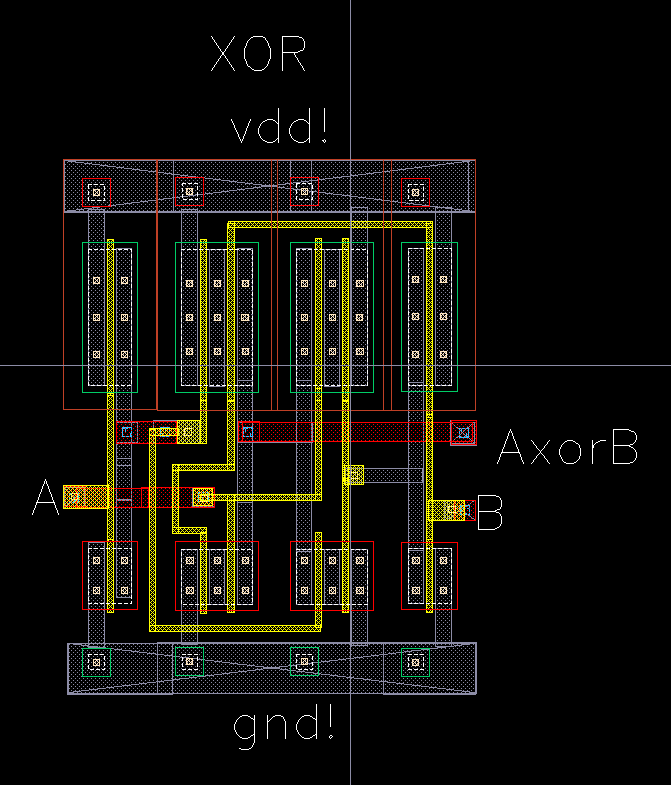
\includegraphics[width = 0.6\linewidth]{xor2_layout.png}
    \caption{Layout of XOR Gate}
    \label{Layout of XOR Gate}
\end{figure}

The performance of XOR Gate is shown in Table \ref{The delay of XOR}.

\begin{table}[h]
    \caption{The delay of XOR Gate}
    \begin{center}
        \begin{tabular}{|c|c|c|c|c|c|c|}
            \hline
            \textbf{Cap} & \multicolumn{2}{|c|}{15f F} & \multicolumn{2}{|c|}{120f F} & \multicolumn{2}{|c|}{960f F} \\
            \hline
            \textbf{State} & Up & Down & Up & Down & Up & Down \\
            \hline
            \textbf{Delay(ns)} & 0.141 & 0.113 & 0.359 & 0.270 & 2.076 & 1.493 \\
            \hline
        \end{tabular}
    \end{center}
    \label{The delay of XOR}
\end{table}

\section{Adder}

For adder, more horizontal wire are required, it is hard to avoid using high level metal wire and the area will be big if we put all the MOS pairs in a line. To solve this problem, we put all the pairs in to two layers, and we also use poly and metal1 as wire as many as possible so we can reduce the area and delay. More importantly we put the pairs in two row, so wiring vertally is possible, which greatly shorten the length of wire. 

\subsection{Half Adder}

% Explain the circuit structure and operation of the half adder that is used in multiplier design. Provide the circuit schematic in the report. Provide the sizes (both width and length in micrometers) of all the transistors.

A half adder is a conbination of a AND Gate and a XOR Gate, each of their input A and B are connected together and the outout of XOR Gate is defined as Sum, the outpt of AND is defined as Carry. The size of the transistors can be refered from XOR Gate and AND Gate introduced before.

\begin{figure}[H]
    \centering
    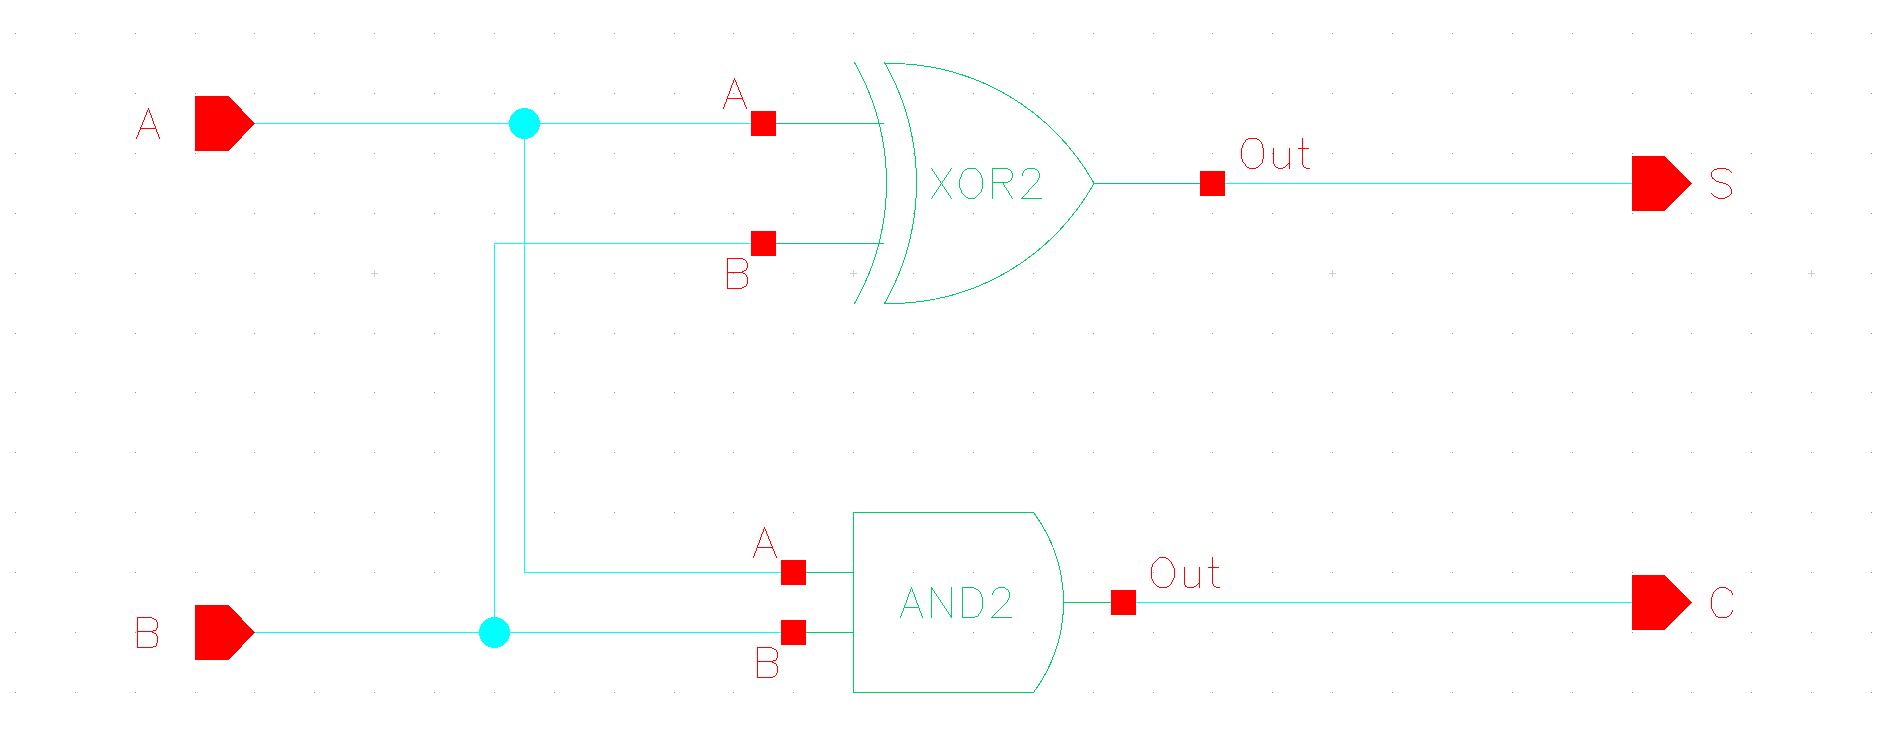
\includegraphics[width = 0.9\linewidth]{half_adder_schematic.png}
    \caption{Schematic of Half Adder}
    \label{Schematic of Half Adder}
\end{figure}

\begin{figure}[H]
    \centering
    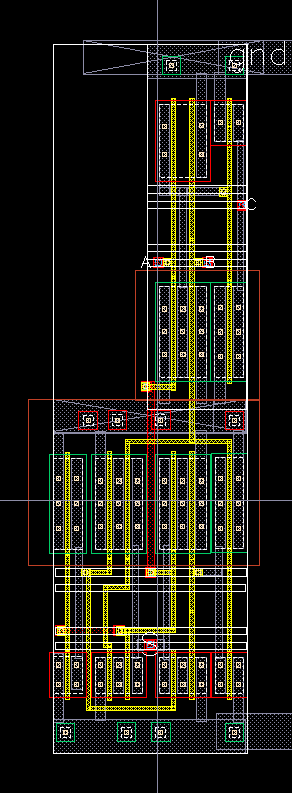
\includegraphics[width = 0.3\linewidth]{half_adder_layout.png}
    \caption{Layout of Half Adder}
    \label{Layout of Half Adder}
\end{figure}
  
\subsection{Full Adder}

% Explain the circuit structure and operation of the full adder that is used in multiplier design. Provide the circuit schematic in the report. Provide the sizes (both width and length in micrometers) of all the transistors.

As shown in Fig \ref{Schematic of Full Adder}, a full adder is a combination of XOR Gates and NAND gates, the structure here is simplified from the classical design in which a full adder contians two half adder and AND Gate, so 

\begin{figure}[H]
    \centering
    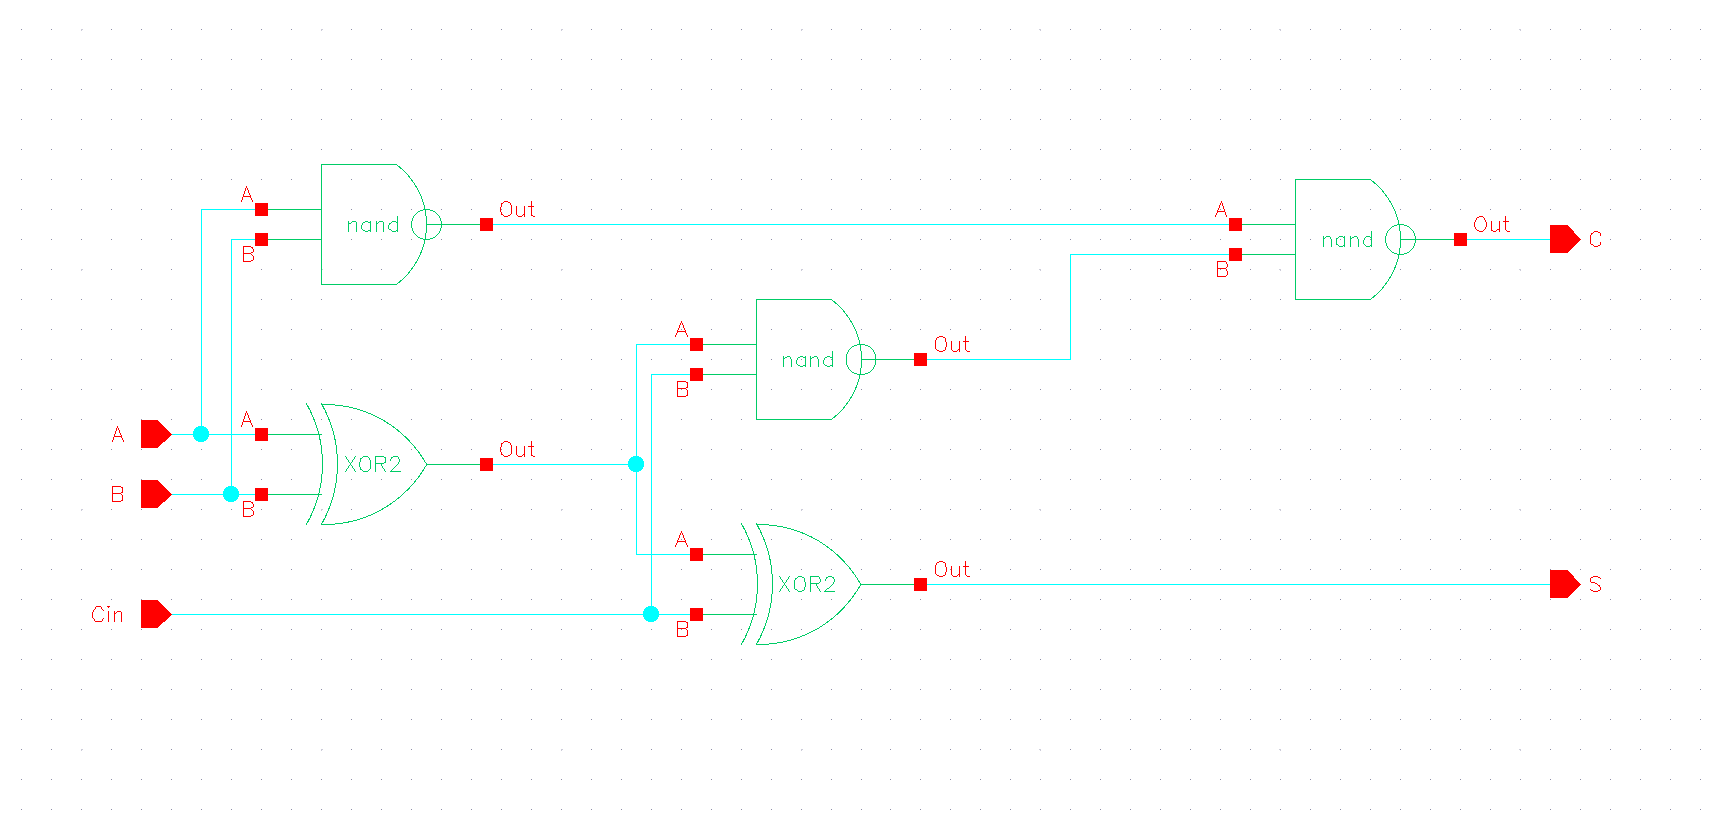
\includegraphics[width = 0.9\linewidth]{full_adder_schematic.png}
    \caption{Schematic of Full Adder}
    \label{Schematic of Full Adder}
\end{figure}
 
\begin{figure}[H]
    \centering
    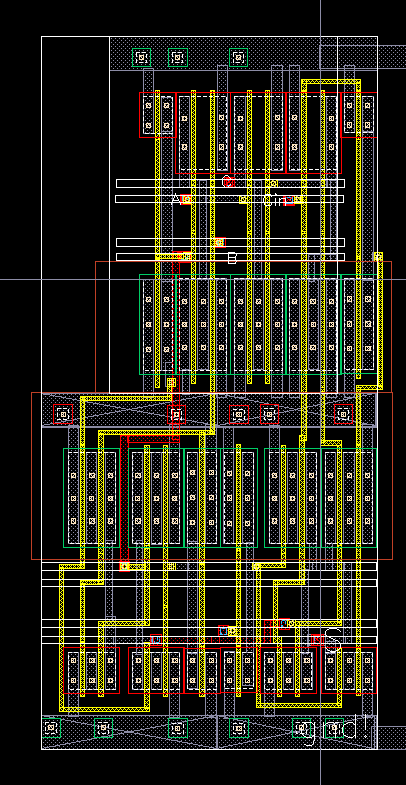
\includegraphics[width = 0.5\linewidth]{full_adder_layout.png}
    \caption{Layout of Full Adder}
    \label{Layout of Full Adder}
\end{figure}


\section{Assemble of the multiplier}
\label{Assemble}

% Explain the structure and operation of the array multiplier. Provide the circuit structure in the report. Clearly label all the inputs and outputs. Clearly show all the connections among various components. Determine the number of critical (longest) delay paths in the 4x4-bit array multiplier. Identify and report the input vectors that excite these critical propagation delay paths. Show one of these critical delay paths on the figure. Measure the propagation delay of the multiplier with schematic level simulation. Assume each product output drives 50 fF extrinsic load capacitor. Report the delays.

\subsection{Schemetic}



\subsection{Layout}

\section{Varication and benckmark of the multiplier}
\label{test}

% Show the layout of your array multiplier in the report. Report the area of your layout. Measure the post-layout propagation delay and report it in your report. Assume each product output drives 50 fF extrinsic load capacitor. Compare the post-layout delay measurements with the schematic level delay measurement. Explain the differences. Discuss the limitations of the schematic level circuit simulation tool. Discuss the importance of accurate resistance and capacitance extraction for correct delay estimation with CADENCE tools.

After we finish the design of the multiplier we need to test the performance of the multiplier.

\subsection{Area of the Layout}

\subsection{propagation delay}

Here we will compare the post-layout delay measurements with the schematic level delay measurement 50f F cap is attached to the output.

\section{Conclusion}

In this project, we experience the procedure of Top to Down design and Down to Top Develop, we first design the multiplier in hignest level, then we gradually split each of the component so we can get the basic logic gate we need. The development procedure start form the bisic logic gate, we design half adder and full adder based on these logic gates, finally the multiplier will be constructed by adders. In each level a serises of test were done to make sure the design functions well. During the layout procedure, we change the way transistors were put, so the size and delay is reduced.


% \section{Ease of Use}

\subsection{Maintaining the Integrity of the Specifications}

The IEEEtran class file is used to format your paper and style the text. All margins, 
column widths, line spaces, and text fonts are prescribed; please do not 
alter them. You may note peculiarities. For example, the head margin
measures proportionately more than is customary. This measurement 
and others are deliberate, using specifications that anticipate your paper 
as one part of the entire proceedings, and not as an independent document. 
Please do not revise any of the current designations.

\section{Prepare Your Paper Before Styling}
Before you begin to format your paper, first write and save the content as a 
separate text file. Complete all content and organizational editing before 
formatting. Please note sections \ref{AA}--\ref{SCM} below for more information on 
proofreading, spelling and grammar.

Keep your text and graphic files separate until after the text has been 
formatted and styled. Do not number text heads---{\LaTeX} will do that 
for you.

\subsection{Abbreviations and Acronyms}\label{AA}
Define abbreviations and acronyms the first time they are used in the text, 
even after they have been defined in the abstract. Abbreviations such as 
IEEE, SI, MKS, CGS, ac, dc, and rms do not have to be defined. Do not use 
abbreviations in the title or heads unless they are unavoidable.

\subsection{Units}
\begin{itemize}
\item Use either SI (MKS) or CGS as primary units. (SI units are encouraged.) English units may be used as secondary units (in parentheses). An exception would be the use of English units as identifiers in trade, such as ``3.5-inch disk drive''.
\item Avoid combining SI and CGS units, such as current in amperes and magnetic field in oersteds. This often leads to confusion because equations do not balance dimensionally. If you must use mixed units, clearly state the units for each quantity that you use in an equation.
\item Do not mix complete spellings and abbreviations of units: ``Wb/m\textsuperscript{2}'' or ``webers per square meter'', not ``webers/m\textsuperscript{2}''. Spell out units when they appear in text: ``. . . a few henries'', not ``. . . a few H''.
\item Use a zero before decimal points: ``0.25'', not ``.25''. Use ``cm\textsuperscript{3}'', not ``cc''.)
\end{itemize}

\subsection{Equations}
Number equations consecutively. To make your 
equations more compact, you may use the solidus (~/~), the exp function, or 
appropriate exponents. Italicize Roman symbols for quantities and variables, 
but not Greek symbols. Use a long dash rather than a hyphen for a minus 
sign. Punctuate equations with commas or periods when they are part of a 
sentence, as in:
\begin{equation}
a+b=\gamma\label{eq}
\end{equation}

Be sure that the 
symbols in your equation have been defined before or immediately following 
the equation. Use ``\eqref{eq}'', not ``Eq.~\eqref{eq}'' or ``equation \eqref{eq}'', except at 
the beginning of a sentence: ``Equation \eqref{eq} is . . .''

\subsection{\LaTeX-Specific Advice}

Please use ``soft'' (e.g., \verb|\eqref{Eq}|) cross references instead
of ``hard'' references (e.g., \verb|(1)|). That will make it possible
to combine sections, add equations, or change the order of figures or
citations without having to go through the file line by line.

Please don't use the \verb|{eqnarray}| equation environment. Use
\verb|{align}| or \verb|{IEEEeqnarray}| instead. The \verb|{eqnarray}|
environment leaves unsightly spaces around relation symbols.

Please note that the \verb|{subequations}| environment in {\LaTeX}
will increment the main equation counter even when there are no
equation numbers displayed. If you forget that, you might write an
article in which the equation numbers skip from (17) to (20), causing
the copy editors to wonder if you've discovered a new method of
counting.

{\BibTeX} does not work by magic. It doesn't get the bibliographic
data from thin air but from .bib files. If you use {\BibTeX} to produce a
bibliography you must send the .bib files. 

{\LaTeX} can't read your mind. If you assign the same label to a
subsubsection and a table, you might find that Table I has been cross
referenced as Table IV-B3. 

{\LaTeX} does not have precognitive abilities. If you put a
\verb|\label| command before the command that updates the counter it's
supposed to be using, the label will pick up the last counter to be
cross referenced instead. In particular, a \verb|\label| command
should not go before the caption of a figure or a table.

Do not use \verb|\nonumber| inside the \verb|{array}| environment. It
will not stop equation numbers inside \verb|{array}| (there won't be
any anyway) and it might stop a wanted equation number in the
surrounding equation.

\subsection{Some Common Mistakes}\label{SCM}
\begin{itemize}
\item The word ``data'' is plural, not singular.
\item The subscript for the permeability of vacuum $\mu_{0}$, and other common scientific constants, is zero with subscript formatting, not a lowercase letter ``o''.
\item In American English, commas, semicolons, periods, question and exclamation marks are located within quotation marks only when a complete thought or name is cited, such as a title or full quotation. When quotation marks are used, instead of a bold or italic typeface, to highlight a word or phrase, punctuation should appear outside of the quotation marks. A parenthetical phrase or statement at the end of a sentence is punctuated outside of the closing parenthesis (like this). (A parenthetical sentence is punctuated within the parentheses.)
\item A graph within a graph is an ``inset'', not an ``insert''. The word alternatively is preferred to the word ``alternately'' (unless you really mean something that alternates).
\item Do not use the word ``essentially'' to mean ``approximately'' or ``effectively''.
\item In your paper title, if the words ``that uses'' can accurately replace the word ``using'', capitalize the ``u''; if not, keep using lower-cased.
\item Be aware of the different meanings of the homophones ``affect'' and ``effect'', ``complement'' and ``compliment'', ``discreet'' and ``discrete'', ``principal'' and ``principle''.
\item Do not confuse ``imply'' and ``infer''.
\item The prefix ``non'' is not a word; it should be joined to the word it modifies, usually without a hyphen.
\item There is no period after the ``et'' in the Latin abbreviation ``et al.''.
\item The abbreviation ``i.e.'' means ``that is'', and the abbreviation ``e.g.'' means ``for example''.
\end{itemize}
An excellent style manual for science writers is \cite{b7}.

\subsection{Authors and Affiliations}
\textbf{The class file is designed for, but not limited to, six authors.} A 
minimum of one author is required for all conference articles. Author names 
should be listed starting from left to right and then moving down to the 
next line. This is the author sequence that will be used in future citations 
and by indexing services. Names should not be listed in columns nor group by 
affiliation. Please keep your affiliations as succinct as possible (for 
example, do not differentiate among departments of the same organization).

\subsection{Identify the Headings}
Headings, or heads, are organizational devices that guide the reader through 
your paper. There are two types: component heads and text heads.

Component heads identify the different components of your paper and are not 
topically subordinate to each other. Examples include Acknowledgments and 
References and, for these, the correct style to use is ``Heading 5''. Use 
``figure caption'' for your Figure captions, and ``table head'' for your 
table title. Run-in heads, such as ``Abstract'', will require you to apply a 
style (in this case, italic) in addition to the style provided by the drop 
down menu to differentiate the head from the text.

Text heads organize the topics on a relational, hierarchical basis. For 
example, the paper title is the primary text head because all subsequent 
material relates and elaborates on this one topic. If there are two or more 
sub-topics, the next level head (uppercase Roman numerals) should be used 
and, conversely, if there are not at least two sub-topics, then no subheads 
should be introduced.

\subsection{Figures and Tables}
\paragraph{Positioning Figures and Tables} Place figures and tables at the top and 
bottom of columns. Avoid placing them in the middle of columns. Large 
figures and tables may span across both columns. Figure captions should be 
below the figures; table heads should appear above the tables. Insert 
figures and tables after they are cited in the text. Use the abbreviation 
``Fig.~\ref{fig}'', even at the beginning of a sentence.

\begin{table}[htbp]
\caption{Table Type Styles}
\begin{center}
\begin{tabular}{|c|c|c|c|}
\hline
\textbf{Table}&\multicolumn{3}{|c|}{\textbf{Table Column Head}} \\
\cline{2-4} 
\textbf{Head} & \textbf{\textit{Table column subhead}}& \textbf{\textit{Subhead}}& \textbf{\textit{Subhead}} \\
\hline
copy& More table copy$^{\mathrm{a}}$& &  \\
\hline
\multicolumn{4}{l}{$^{\mathrm{a}}$Sample of a Table footnote.}
\end{tabular}
\label{tab1}
\end{center}
\end{table}

\begin{figure}[htbp]
\centerline{
\includegraphics{fig1.png}}
\caption{Example of a figure caption.}
\label{fig}
\end{figure}

Figure Labels: Use 8 point Times New Roman for Figure labels. Use words 
rather than symbols or abbreviations when writing Figure axis labels to 
avoid confusing the reader. As an example, write the quantity 
``Magnetization'', or ``Magnetization, M'', not just ``M''. If including 
units in the label, present them within parentheses. Do not label axes only 
with units. In the example, write ``Magnetization (A/m)'' or ``Magnetization 
\{A[m(1)]\}'', not just ``A/m''. Do not label axes with a ratio of 
quantities and units. For example, write ``Temperature (K)'', not 
``Temperature/K''.

\section*{Acknowledgment}

The preferred spelling of the word ``acknowledgment'' in America is without 
an ``e'' after the ``g''. Avoid the stilted expression ``one of us (R. B. 
G.) thanks $\ldots$''. Instead, try ``R. B. G. thanks$\ldots$''. Put sponsor 
acknowledgments in the unnumbered footnote on the first page.

\section*{References}

Please number citations consecutively within brackets \cite{b1}. The 
sentence punctuation follows the bracket \cite{b2}. Refer simply to the reference 
number, as in \cite{b3}---do not use ``Ref. \cite{b3}'' or ``reference \cite{b3}'' except at 
the beginning of a sentence: ``Reference \cite{b3} was the first $\ldots$''

Number footnotes separately in superscripts. Place the actual footnote at 
the bottom of the column in which it was cited. Do not put footnotes in the 
abstract or reference list. Use letters for table footnotes.

Unless there are six authors or more give all authors' names; do not use 
``et al.''. Papers that have not been published, even if they have been 
submitted for publication, should be cited as ``unpublished'' \cite{b4}. Papers 
that have been accepted for publication should be cited as ``in press'' \cite{b5}. 
Capitalize only the first word in a paper title, except for proper nouns and 
element symbols.

For papers published in translation journals, please give the English 
citation first, followed by the original foreign-language citation \cite{b6}.

\begin{thebibliography}{00}
\bibitem{b1} G. Eason, B. Noble, and I. N. Sneddon, ``On certain integrals of Lipschitz-Hankel type involving products of Bessel functions,'' Phil. Trans. Roy. Soc. London, vol. A247, pp. 529--551, April 1955.
\bibitem{b2} J. Clerk Maxwell, A Treatise on Electricity and Magnetism, 3rd ed., vol. 2. Oxford: Clarendon, 1892, pp.68--73.
\bibitem{b3} I. S. Jacobs and C. P. Bean, ``Fine particles, thin films and exchange anisotropy,'' in Magnetism, vol. III, G. T. Rado and H. Suhl, Eds. New York: Academic, 1963, pp. 271--350.
\bibitem{b4} K. Elissa, ``Title of paper if known,'' unpublished.
\bibitem{b5} R. Nicole, ``Title of paper with only first word capitalized,'' J. Name Stand. Abbrev., in press.
\bibitem{b6} Y. Yorozu, M. Hirano, K. Oka, and Y. Tagawa, ``Electron spectroscopy studies on magneto-optical media and plastic substrate interface,'' IEEE Transl. J. Magn. Japan, vol. 2, pp. 740--741, August 1987 [Digests 9th Annual Conf. Magnetics Japan, p. 301, 1982].
\bibitem{b7} M. Young, The Technical Writer's Handbook. Mill Valley, CA: University Science, 1989.
\end{thebibliography}
\vspace{12pt}
\color{red}
IEEE conference templates contain guidance text for composing and formatting conference papers. Please ensure that all template text is removed from your conference paper prior to submission to the conference. Failure to remove the template text from your paper may result in your paper not being published.



\begin{thebibliography}{01}
    \bibitem{a1} S. Kumar, ‘A Review of Different Type of Multipliers and Multiplier-Accumulator Unit.’, vol. 2, no. 4, p. 5, 2013.

    \bibitem{a2} N. Maheshwari, ‘A Design of 4X4 Multiplier using 0.18 um Technology’, International Journal of Latest Trends in Engineering and Technology, vol. 2, no. 1, p. 7, 2013.
    \bibitem{a3} M. Krishnamurthy, ‘A. Joseph vijay1, Scholar, Department of’, p. 10.
    \bibitem{a4} N. Singh and M. Z. Alam, ‘Design and Implementation of Pipelined 4-Bit Binary Multiplier Using M.G.D.I. Technique’, Management Research, vol. 2, no. 3, p. 7, 2014.
    \bibitem{a5} ‘Design of Low Power and High Speed 4X4 Multiplier using Modified Column Bypassing Scheme for DSP Applications’, ijrte, vol. 8, no. 2S3, pp. 643–647, Aug. 2019, doi: 10/gj4nkd.
    \bibitem{a6} M. H. Riaz, S. A. Ahmed, Q. Javaid, and T. Kamal, ‘Low power 4×4 bit multiplier design using dadda algorithm and optimized full adder’, in 2018 15th International Bhurban Conference on Applied Sciences and Technology (IBCAST), Islamabad, Jan. 2018, pp. 392–396. doi: 10/gj4nkf.
    \bibitem{a7} S. Agwa, E. Yahya, and Y. Ismail, ‘Variability mitigation using correction function technique’, in 2013 IEEE 20th International Conference on Electronics, Circuits, and Systems (ICECS), Abu Dhabi, United Arab Emirates, Dec. 2013, pp. 293–296. doi: 10/gj4nkg.

\end{thebibliography}

\end{document}
